\documentclass[11pt]{article}
\usepackage[a4paper,top=22mm,bottom=23mm,left=23mm,right=23mm]{geometry}
\usepackage{amsmath,amssymb,booktabs,array,graphicx,xcolor,hyperref,fancyhdr}
\definecolor{teal}{HTML}{09646A}
\definecolor{ink}{HTML}{24343D}
\hypersetup{colorlinks=true,urlcolor=teal,citecolor=teal,linkcolor=teal,pdftitle={When does a crop camera benefit from paying for labels?}}
\pagestyle{fancy}\fancyhf{}\fancyhead[L]{\footnotesize\textcolor{teal}{EDGE AI \enspace / \enspace FIELD IMAGE TRIAGE}}
\fancyhead[R]{\footnotesize Research manuscript}\fancyfoot[C]{\small\thepage}
\setlength{\headheight}{15pt}\setlength{\parindent}{0pt}\setlength{\parskip}{5pt}
\setlength{\tabcolsep}{6pt}\renewcommand{\arraystretch}{1.16}
\newcommand{\sect}[1]{\vspace{3pt}\noindent{\large\bfseries\color{teal}#1}\par}
\newcommand{\subt}[1]{\smallskip\noindent{\bfseries #1}\par}
\newcommand{\note}[1]{{\footnotesize\emph{#1}\par}}
\newcommand{\BA}{\mathrm{BA}}
\urlstyle{same}
\begin{document}
{\footnotesize\color{teal}\bfseries RESEARCH ARTICLE \hfill WORKING DRAFT \quad 27 NOVEMBER 2026}\par
\vspace{4mm}
{\LARGE\bfseries When does a crop camera benefit\\[2pt] from paying for labels?}\par
{\large\color{ink}A byte-matched evaluation of online edge--cloud review across apple-leaf collections}\par
\vspace{3mm}
\sect{Abstract}
A crop camera can spend a limited connection on two competing actions: send calibration images for expert annotation and install a new prediction head, or keep its classifier and upload selected observations for review. We compare these actions using real encoded messages, two edge models, a common cloud expert and three image collections. Our primary replay gives a camera a fixed quota before deployment, charges remote annotation to that quota and permits one compressed frame at a time. With 32 calibration labels, the updated MobileNetV2 system reaches 83.03\%, 80.44\% and 53.16\% balanced accuracy on Cornell, Kashmir and Latvia, respectively. With 128 labels it reaches 84.52\%, 73.32\% and 53.54\%. The larger update exhausts the available setup allowance on every Kashmir draw. Under a common online controller, the binary EdgeBoost confidence score produces identical queries to our simple margin, and a published learned deferral rule performs better on Cornell. With MobileNetV4, updating before review improves on frozen-camera review only on Cornell at the retrospective 25\% byte ceiling. On the Latvian scab task, 84.6\% of the extra missed positives arise before an image is sent. These finite-cohort results quantify when paying for a new classifier helps, when the camera should keep its existing head, and how proxy hardware and the definition of disease limit both conclusions.

\sect{1 \quad The decision at the gateway}
A remote annotator must usually see the leaf before supplying its label. At what point does buying that label leave too little capacity for subsequent alerts? A second uncertainty is the order of arrivals. The camera must decide whether to send the present frame while the severity, scores and JPEG lengths of future frames are unknown. A third is the value of the reply: forwarding a difficult frame helps only if the cloud expert can correct the camera.

Previous work quantified the gap between controlled and field photographs \cite{mohanty}, confidence-based deferral \cite{jit,edgeboost}, embedded updates \cite{tinyol,lin} and scheduling of model specialization on edge GPUs \cite{ekya,remembrall}. We connect the cost of acquiring supervision to the subsequent review decisions. All paired comparisons within each protocol share evaluation identities, the available label draw, the cloud expert and an absolute byte allowance. We trace changes in both false alarms and missed disease. A test against the expert's source-specific reference for a single photograph cannot establish plant health or crop yield.

\newpage
\sect{2 \quad Inputs, models and comparisons}
\subt{Device measurements and image sources}
AgriTinyVision exposes a 160-pixel binary MobileNetV2 and an archived ESP32-S3 INT8 replay \cite{agri}. We joined all 60 board records to PlantDoc source files by identity, checked the hashes of the actual RGB inputs and repeated the FP32 forward pass. Its maximum probability difference from the archived FP32 result was $5.1\times10^{-7}$ and every three-state output matched. We use the published disease-score threshold of 0.30 for forced binary decisions. The upstream band from 0.20 to below 0.40 allows abstention. The main V2 experiments use its exported FP32 backbone on a CPU. We also replay the released ESP-PPQ tensor scales on the host and repeat the evaluation with a MobileNetV4 pipeline. The original 60 records are the only physical-device observations. PlantDoc images were sourced from the internet \cite{singh}.

\begin{center}\small
\begin{tabular}{@{}>{\raggedright\arraybackslash}p{34mm}rp{99mm}@{}}\toprule
Evidence & Images & Role in the comparisons\\\midrule
PlantDoc board replay & 60 & Historical device outputs for 15 source classes across four crops.\\
PlantDoc target crops & 131 & All eligible official test images. A decontaminated comparison retains 121, including 66 outside the archived board subset and its duplicate components.\\
Cornell FGVC7 & 1,821 & Expert-labelled apple images. Used as released for frozen inference. A separate target-assisted protocol draws from 450 representatives and tests on 1,353 remaining representatives.\\
Kashmir stress pool & 384 & Fixed hash sample of 128 images per released class. Every applied head was fitted elsewhere.\\
Latvian orchard & 1,190 & Whole public archive with scab labels. Used for external replay and a separate early-to-late-date calibration experiment.\\\bottomrule
\end{tabular}\end{center}

We audited published splits, hashes and candidate near-duplicates. Fourteen of 236 official PlantDoc test files matched training files. Cornell \cite{thapa} had no match against 5,370 audited upstream files at perceptual-hash distance at most four. Image identity screens cannot establish plant-level independence. Kashmir's processed sample lacks parent-leaf identifiers.

\subt{A byte-identical remote comparison}
We encode oriented images as quality-75 JPEGs at a maximum long edge of 224 pixels. The primary expert is a frozen DINOv2-small \cite{dino} with a class-balanced logistic head fitted to 1,237 distinct PlantDoc training payloads (190 healthy). The same decoded JPEG reaches the same expert for every matched routing policy. Appendix A includes 112-pixel payloads, an independently pretrained MobileNetV2 \cite{mobile}, and an unweighted DINO head. We report balanced accuracy, $\BA=(\mathrm{sensitivity}+\mathrm{specificity})/2$, supplemented by false alarms, misses and ordinary accuracy.

\subt{Shared calibration and service contract}
For V2, 20 seeded draws of 32 or 128 labels come from a 450-image Cornell calibration bank that excludes all holdout components. The device transmits a signed-byte 1,280-dimensional activation with its scale, label and identifier (1,293 bytes per record). A class-balanced logistic head is returned in 1,294 bytes. The source-trained remote service receives a 224-pixel JPEG with 20 bytes of application fields per query. A cold start charges setup against the same quota as serving. Prepaid results isolate inference after setup and are reported separately. The online replay fixes the quota before the first arrival. The retrospective scheduler instead prices its cap from the complete test batch. Its access to future scores and lengths defines a different scheduling problem.

\newpage
\sect{3 \quad One-frame routing with remotely acquired labels}
Can a camera afford to update its classifier and still send useful photographs as they arrive? We charge each Cornell calibration JPEG sent for human annotation, its feature record, the returned head, and subsequent uploads to the same allowance. At the start of a window with $N$ scheduled arrivals, the camera receives $B=\lfloor Nq\bar b\rfloor$ application bytes. The planning mean $\bar b$ uses the first 32 calibration JPEGs plus 20 bytes per transaction in each draw. At $q=0.25$, the mean grants for Cornell, Kashmir and Latvia are 2,273,844, 645,348 and 1,999,907 bytes, respectively (24.87\%, 17.06\% and 18.54\% of actual full-review traffic). We also replayed $q=0.10$ and $0.50$.

At each arrival the camera can encode and hold one JPEG. The fixed gate uses a cutoff fitted on calibration images. The paced gate adjusts that cutoff after each arrival using remaining bytes, scheduled arrivals and previously observed candidate sizes. Neither gate sees future scores. Latvia follows capture timestamps across 14 dates. Cornell and Kashmir lack usable capture timestamps, so we average five deterministic image-hash orders per draw. Human turnaround time and codec workspace are outside this replay. Checksums and lengths matched for all 2,927 encoded JPEGs. The largest individual payload was 13,205 bytes.

\begin{center}\small
{\renewcommand{\arraystretch}{1.03}\begin{tabular}{@{}lrrrr@{}}\toprule
Mean balanced accuracy (\%), $q=0.25$ & Labels & Cornell & Kashmir & Latvia\\\midrule
\multicolumn{5}{@{}l}{\emph{A. Same 20 calibration draws, remote acquisition charged}}\\
Updated camera alone & 32 &77.35&77.29&51.12\\
Updated camera, fixed cutoff &32&82.06&80.09&53.35\\
Updated camera, paced cutoff &32&83.03&80.44&53.16\\
Updated camera alone &128&80.01&67.58&52.11\\
Updated camera, fixed cutoff &128&83.51&73.93&52.80\\
Updated camera, paced cutoff &128&84.52&73.32&53.54\\\midrule
\multicolumn{5}{@{}l}{\emph{B. Published routing scores, shared one-frame percentile gate except last row}}\\
Original camera uncertainty &128&72.33&73.13&50.26\\
Updated camera uncertainty &128&84.47&73.13&53.26\\
EdgeBoost margin &128&84.47&73.13&53.26\\
CompareConfidence &128&84.84&73.13&53.37\\
One-vs-all deferral &128&85.00&73.13&53.57\\
Mao et al.\ two-stage deferral &128&83.48&73.13&53.32\\
EdgeBoost, calibrated fixed cutoff &128&84.55&73.13&54.00\\\bottomrule
\end{tabular}}\end{center}

With 32 labels, pacing adds 5.68 points over the updated camera on Cornell and 3.15 on Kashmir. Every 32-label update fits. Every 128-label update exceeds the Kashmir allowance and falls back to the original camera. On Latvia, 128-label pacing gives 53.54\% balanced accuracy with 496.4 missed scab cases per draw, versus 118 for the original camera. A stricter policy earns $q\bar b$ bytes per arrival from zero initial credit and saves for installation. Its 128-label results fall to 78.16\%, 67.58\% and 45.35\%, respectively.

Panel B isolates the routing score. After 16 unqueried arrivals, the gate ranks each score against up to 64 past scores, then applies the funded fraction of remaining arrivals. CompareConfidence, one-vs-all and two-stage deferral \cite{cc,ova,mao} use class-balanced linear heads on frozen features, the same 128 images and server, and paid router weights. For a binary logit $z$ and temperature $T>0$, EdgeBoost's margin \cite{edgeboost} $\tanh(|z|/(2T))$ preserves the uncertainty ordering. Both scores produced identical query masks in all 1,320 paired comparisons. EdgeBoost's separate calibration-fitted cutoff retains its original threshold semantics under the same hard cap. One-vs-all led Cornell by 0.53 points over updated uncertainty, while the EdgeBoost cutoff led Latvia by 0.74 points. The experiment supports the value of camera adaptation on Cornell and the affordable Kashmir draws. It provides no evidence of a superior new routing score.

\newpage
\sect{4 \quad Published routing methods at the same byte ceiling}
We compared published routing rules on the same edge features, remote classifier and test images. Each of 20 draws supplied precisely 128 Cornell labels. All inference queries sent a measured 224-pixel quality-75 JPEG and 20 protocol bytes. This retrospective, batch-sorted comparison used a ceiling of 25\% of the cost of querying every image in the cohort. In the cold-start settings, we debited installation before allocating test queries. Remote annotation required calibration JPEGs, which could also supply expert supervision. The prepaid setting gave every installed router the same inference budget. A router that exceeded its allowance fell back to an affordable updated head, then to the source head if necessary.

\begin{center}\begingroup\footnotesize\setlength{\tabcolsep}{2.8pt}
\begin{tabular}{@{}lrrrrrrrrr@{}}\toprule
&\multicolumn{3}{c}{Cold, local labels}&\multicolumn{3}{c}{Cold, remote labels}&\multicolumn{3}{c}{Prepaid}\\
\cmidrule(lr){2-4}\cmidrule(lr){5-7}\cmidrule(lr){8-10}
AgriTinyVision edge, mean BA (\%) & C & K & L & C & K & L & C & K & L\\\midrule
Updated confidence / EdgeBoost rank&87.06&84.28&54.74&84.76&76.37&53.70&87.26&85.09&54.86\\
EdgeBoost fixed gate&86.31&83.14&54.05&84.34&76.37&53.47&86.45&84.19&54.19\\
OvA, class-balanced&85.30&84.28&54.08&85.30&76.37&54.08&87.43&84.98&55.70\\
CompareConfidence, balanced&85.25&84.28&53.73&85.25&76.37&53.73&87.54&85.11&55.22\\
Two-stage cost, balanced&83.71&84.28&53.49&83.71&76.37&53.49&84.58&82.27&53.81\\
Diff-01, 20 epochs&82.17&84.28&53.71&82.17&76.37&53.71&83.05&82.62&55.07\\
Diff-Prob, 20 epochs&83.41&84.28&53.80&83.41&76.37&53.80&84.52&80.71&55.23\\
Gatekeeper, $\alpha=.5$&81.11&81.78&53.10&78.58&76.37&51.93&81.75&82.82&53.45\\
Balanced CE continuation&87.69&84.42&55.41&85.93&76.37&54.38&87.97&85.39&55.64\\
\bottomrule\end{tabular}\endgroup\end{center}
{\footnotesize C, K and L denote Cornell ($n=1{,}353$), Kashmir ($384$) and Latvia ($1{,}190$). In Kashmir, cold-start routers requiring all 128 expert outputs could afford only the updated confidence fallback with local labels, or the source-camera fallback with remote labels. The full-feedback learned-router entries include these fallbacks.\par}

Said and Landsiedel's EdgeBoost (\emph{Computer Networks}, 2025)\,\cite{edgeboost} accepts a confident local prediction using a temperature-calibrated top-two probability gap. On the authors' 8,000 stored CIFAR cases, our gate matched their implementation at all seven reported thresholds. For two classes and positive temperature $T$, the gap is $\tanh(|z|/(2T))$, where $z$ is the signed edge logit. Ordering a buffered batch by this gap therefore yields the same ranking as ordering by $|z|$. Across 360 charged operating points, both rankings selected exactly the same images and produced identical decisions. A separately calibrated fixed-threshold gate retained the original threshold semantics and could leave bytes unused.

Verma and Nalisnick's OvA (ICML 2022)\,\cite{ova} and CompareConfidence as implemented by Mozannar et al.\ (AISTATS 2023)\,\cite{cc} compare expert correctness with local class scores. Our binary linear ports share fitted heads and apply different score transformations. Mao et al.'s two-stage cost-sensitive surrogate (ICML 2025)\,\cite{mao} uses out-of-fold local errors and measured cloud errors. The table reports equal class weights in the risk aggregate through inverse-frequency sample weighting, matching balanced accuracy. As a feedback-cost sensitivity, CompareConfidence with all 128 true labels and only 32 expert outputs achieved 86.79/83.27/54.48\% under cold local accounting. With full feedback prepaid, its mean gains over updated confidence were 0.28, 0.02 and 0.36 percentage points. Ties in these learned scores used salted image identifiers to prevent label names in public paths from determining uploads.

Jitkrittum et al.'s Diff-01 and Diff-Prob (NeurIPS 2023)\,\cite{jit} regress the expert's advantage in correctness or true-class probability. We specialized their probability features to two classes and used four-fold local predictions. Twenty epochs on 128 calibration pictures give only 20 full-batch updates. An 800-step, class-balanced sensitivity reached 87.28/83.52/55.84\% for prepaid Diff-Prob. Rabanser et al.'s Gatekeeper (NeurIPS 2025)\,\cite{gate} applies cross-entropy to correct predictions and a penalty for deviation from uniform confidence to errors. We tuned its final layer for 100 steps on the shared labels. Ordinary class-balanced cross-entropy (CE) for the same 100 steps beat the basic confidence rule at identical cold local cost in all three cohorts.

\begin{samepage}\medskip\noindent\textbf{A second edge model.}
We repeated the experiment using MobileNetV4-Conv-Small (Qin et al., ECCV 2024)\,\cite{vfour}, with public ImageNet weights, the model's 224-pixel preprocessing and a binary head trained on 1,237 PlantDoc source images. We verified all 4,632 original image digests and reconstructed the graph's ImageNet logits from the extracted activations to within $6.9\times10^{-5}$. The 1,280-dimensional representation cost 1,293 bytes per calibration record. The final head occupied 1,294 bytes. The V4 and AgriTinyVision systems differ in source training and preprocessing as well as architecture. These V4 measurements cover CPU graph inference and application traffic.\par\end{samepage}

\begin{center}\begingroup\small\setlength{\tabcolsep}{4pt}
\begin{tabular}{@{}lrrrr@{}}\toprule
MobileNetV4, cold BA (\%) & Cornell & Kashmir & Latvia & Latvia, later\\
\midrule
Source head alone&73.23 / 73.23&73.44 / 73.44&66.20 / 66.20&69.28 / 69.28\\
Source head + confidence&80.53 / 80.53&83.59 / 83.59&66.58 / 66.58&68.11 / 68.11\\
Updated head alone&80.73 / 80.73&72.25 / 73.44&58.38 / 58.38&60.49 / 60.49\\
Updated head + random&81.52 / 81.19&74.38 / 75.38&58.98 / 58.71&61.04 / 60.78\\
Updated head + confidence&84.65 / 83.61&76.27 / 83.59&59.40 / 58.98&61.82 / 60.66\\
Gatekeeper&74.42 / 66.45&75.61 / 83.59&59.39 / 56.66&61.66 / 52.56\\
Balanced CE continuation&84.89 / 83.85&77.91 / 83.59&59.82 / 59.59&62.19 / 61.25\\
\bottomrule\end{tabular}\endgroup\end{center}
{\footnotesize Each cell gives local / remote annotation. The later Latvian subset contains 579 of the 1,190 photos. Random review averages 20 fixed orders per calibration draw. All V4 treatments used the same 224-pixel DINO service and the same Cornell calibration identities as above.\par}

With local labels, V4 updating plus confidence routing improved on source-head routing by 4.11 percentage points on Cornell and lost 7.32 points on Kashmir and 7.18 points on Latvia. Paired 95\% resampling intervals were $[1.90,6.37]$, $[-11.62,-2.98]$ and $[-11.44,0.37]$ points, respectively. We resampled pictures within class in Cornell and Kashmir, and whole acquisition dates in Latvia, holding fitted heads and routing decisions fixed. The 20 calibration draws reuse each test pool. The transfer estimates apply to these photographed cohorts.

\newpage
\sect{5 \quad Why does the Latvian system miss visible scab?}
\subt{Separate the updated prediction from the decision to send}
We hold the camera, cloud expert, image identities and per-image JPEG costs fixed within each counterfactual. This diagnostic uses the retrospective 25\% ceiling and charges 166,798 bytes for the update with available labels. Of 983 scab-positive photographs, the released camera misses 118. The Cornell-trained head alone misses 471.80 on average. Reviewing its uncertain predictions with the PlantDoc expert increases misses to 536.35. Thus 353.80 of the 418.35 additional misses (84.6\%) occur before routing. On the transmitted set the server rescues 25.50 misses and introduces 90.05. It removes 25.95 false positives and introduces 1.50. Total false alarms fall from 195 to 74.45. BA thus rises from 46.90\% to 54.74\% even while ordinary accuracy falls from 73.70\% to 48.67\%. The selected camera decisions are correct on 53.66\% of sent images, the cloud's replacements on 38.92\%.

\begin{center}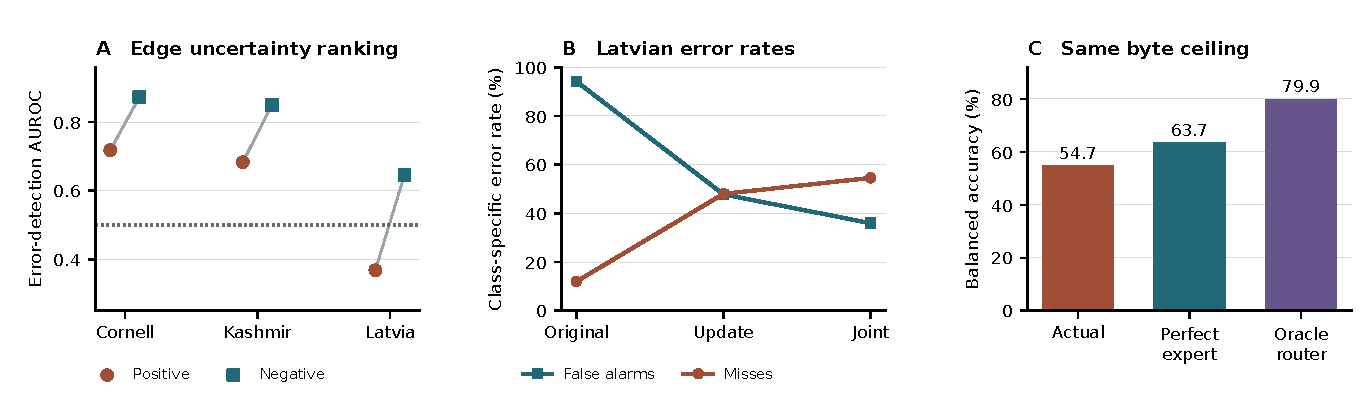
\includegraphics[width=.97\linewidth]{figures/latvia_failure.pdf}\end{center}
\note{Figure 1. Error-detection AUROC conditions on the indicated true class. The stage counts identify when additional misses occur. The label-aware routing ceiling holds both classifiers and the byte allowance fixed. Its access to truth makes it an unattainable deployment reference.}

\subt{A changed endpoint and a changed source}
Cornell's negative class is explicitly healthy. Latvia's negative class means no visible scab and can contain other damage. Restricting Cornell to its 450 scab and 377 healthy evaluation images brings the positive endpoints closer. The updated head's disease-score AUROC is 0.905 on this restriction and 0.528 on Latvia. The frozen server gives 0.955 and 0.696. Changing the positive prevalence alone cannot produce this within-class ranking loss. Restricting Latvian comparisons to positive--negative pairs from the same camera model and date gives edge AUROC 0.512 and cloud AUROC 0.666, covering 8.38\% of possible pairs across eleven mixed strata. We lack common independent labels for scab and any disease on the same Latvian leaves. Acquisition, orchard, severity and residual endpoint differences therefore remain confounded.

Uncertainty detects errors on positive Latvian leaves with AUROC 0.368. It assigns higher priority to many correct positive calls than to misses. At the same cost, a truth-aware router selecting among the actual edge and cloud answers could reach 79.95\% BA, versus 54.74\% for the margin. After removing near-duplicates, margin and random uploads give 54.570\% and 54.526\%, respectively. This is a failure of the available ranking and the expert on its selected cases, even though some affordable frames could have been repaired.

\newpage
\subt{Resolution and site-specific heads}
Keeping the DINO weights, threshold and crop rule fixed, we decoded all 1,190 images from each candidate payload. Full-review AUROC improves from 0.696 at 224 pixels to 0.743 at 448 and 0.757 using the original camera files. Even the latter yields 637 missed scab cases. With the original query identities, the camera--cloud BA improves from 54.74\% to 55.72\% and 55.79\%. With the original \emph{byte} allowance, however, 448 pixels admits 90.5 queries instead of 271.8, lowering BA to 53.30\%. Camera originals admit one query on average and give 52.14\%. This intervention holds the trained classifier fixed and separates loss of visual information from the price of sending it.

We also fit separate edge and server heads using the same 128 early Latvian labels per draw and evaluate only the 579 later images (507 scab, 72 negative). The 25\% inference allowance is identical and setup is prepaid to isolate each component. In the table, the two entries for a given edge head use exactly the same query identities.
\begin{center}\small
\begin{tabular}{@{}llrrr@{}}\toprule
Edge head & Server head & False alarms & Misses & BA (\%)\\\midrule
Cornell & PlantDoc & 23.80 & 267.80 & 57.06\\
Cornell & Early Latvia & 29.70 & 216.65 & 58.01\\
Early Latvia & PlantDoc & 37.35 & 201.40 & 54.20\\
Early Latvia & Early Latvia & 42.35 & 146.70 & 56.12\\\bottomrule
\end{tabular}\end{center}
With every later image reviewed, refitting the server raises its BA from 63.09\% to 68.11\%. Changing both heads brings down missed cases but increases the false alarms among the 72 negatives. The small number of negative dates limits extrapolation to other seasons.

\sect{6 \quad Device and link sensitivity}
\subt{From exported FP32 features to the released INT8 scales}
We replayed the model's recorded ESP-PPQ tensor scales on the CPU using signed quantization and the S3 rounding rule \cite{esp}. For the embedded fixture the host gives output codes $(56,-62)$ versus $(58,-59)$ in the release. It matches 59 of 60 archived binary board decisions, with median absolute disease-probability difference 0.000172 and a maximum of 0.204. This measures numerical sensitivity rather than certifying hardware parity.

On the three evaluation cohorts, median cosine similarity between approximate INT8 and FP32 features is 0.894, 0.908 and 0.918. Holding the FP32-fitted head fixed gives joint BA of 78.86\%, 77.73\% and 50.39\% under remote annotation and the retrospective 25\% ceiling. The FP32 reference gives 84.76\%, 76.37\% and 53.70\%. Retraining the heads on the simulated activations gives 81.60\%, 77.73\% and 53.26\%. For Kashmir the update cannot fit and these comparisons use their respective frozen-camera fallbacks. The approximation can therefore shift predictions enough to affect the operating recommendation. Deployed feature tensors and the latency, total RAM and energy of the new head on an ESP32-S3 remain unmeasured.

\newpage
\subt{An alert deadline changes the value of sending an image}
We distinguish link measurements from assumed operating conditions. Nine public Norwegian forest private-5G measurements provide average uplink goodput (8--179 Mbit/s), downlink goodput (133.4--624 Mbit/s) and RTT (12--27 ms) at different distances \cite{forest}. They are snapshots, without packet arrival times. We replay the same byte-selected queries across each snapshot, add one RTT on an existing connection or three for a cold connection, and budget 0.1 or 0.5 s for cloud work. Late replies preserve the local classification. This separately probes delivery of the retrospective selection. The online routing evaluation in Section 3 assumes replies from funded requests are available.

Under remote 128-label setup, the Cornell camera requests 166.4 reviews on average. All arrive within 2 s in the nine snapshot replays with a 5 s acquisition interval. A separate synthetic link runs at 10/20 kbit/s up/down, RTT 1.2 s, independent 10\% segment loss, up to five attempts, and 60 s out of service every 120 s. At a 2 s deadline none return in time (80.01\% BA). With an existing connection, 0.1 s cloud work and a 30 s deadline, 85.0 arrive on time (82.36\% BA), compared with 84.76\% if every requested reply counts. Expert time is additional: at assumed sequential service of 15 or 60 s per calibration image, 128 labels require 32 or 128 minutes of labor. The link and time assumptions are sensitivities; none is a new measurement from an orchard, an NB-IoT carrier or a human annotator.

\sect{7 \quad What the evidence supports}
For an operator who must send calibration photographs, 32 labels used the nominal online allowance more effectively than 128 in Kashmir, whereas 128 gave the largest of the two mean scores in Cornell. A separate exact cost comparison on Cornell asks how much a truth-aware router must spend to match the updated head alone. The update costs 166,798 bytes with all 128 labels already available, versus 1,026,890 on average when all 128 photographs must be sent. The update is cheaper in 20/20 draws with local labels, 9/20 when 32 of the 128 photographs must be sent, and 0/20 from 64 sent onward in this nested comparison. This bound is specific to the fixed menu in Appendix C. The answer depends on the camera's starting classifier as well as annotation access.

The binary uncertainty score has the same ordering as EdgeBoost with a positive temperature. Matched learned alternatives and a simple cross-entropy control can equal or improve on its results. Across sources, the updated camera assigns low uncertainty to many scab-positive images it misses. The study's contribution is a reproducible set of cost and failure comparisons. The experiments neither establish a superior general routing algorithm nor verify an end-to-end field deployment. A matched dual-label reannotation and board-side feature capture would be needed to identify the remaining endpoint and hardware effects.


\sect{Artifact and provenance}
The accompanying project contains the frozen-experiment specification, per-image decisions and scores, compact fitted heads, aggregate results, source revisions and reconstruction scripts. Obtain the original Cornell references under the competition terms to join the identifiers locally. Raw photographs, restricted feature caches and third-party model weights are obtained separately. It includes the operating-point and source-balancing controls added during analysis. Cornell and Kashmir informed exploratory extensions. The full Latvian archive and chronological holdout were specified before the corresponding outcomes were inspected. There was no public preregistration. The binary labels and pretrained models belong to their original providers. Raw photographs and third-party model weights can be retrieved at their pinned sources. The project includes an independent C99 reader and exhaustive small-pool checks for the cost and audit computations. An AI coding assistant contributed to the computational implementation and drafting. Authorship, affiliations and submission metadata await confirmation by the research team.

\newpage\begingroup\small
\begin{thebibliography}{24}\setlength{\itemsep}{1.5pt}\setlength{\parskip}{0pt}
\bibitem{mohanty} S. P. Mohanty, D. P. Hughes and M. Salathé. Using deep learning for image-based plant disease detection. \emph{Frontiers in Plant Science}, 7, 1419, 2016. \href{https://doi.org/10.3389/fpls.2016.01419}{doi:10.3389/fpls.2016.01419}.
\bibitem{jit} W. Jitkrittum, N. Gupta, A. K. Menon, H. Narasimhan, A. S. Rawat and S. Kumar. When does confidence-based cascade deferral suffice? \emph{NeurIPS}, 2023. \href{https://arxiv.org/abs/2307.02764}{Author manuscript}.
\bibitem{sawade} C. Sawade, N. Landwehr and T. Scheffer. Active comparison of prediction models. \emph{NeurIPS}, 2012. \href{https://proceedings.neurips.cc/paper/2012/hash/92fb0c6d1758261f10d052e6e2c1123c-Abstract.html}{Proceedings}.
\bibitem{musgrove} D. Musgrove, A. Radtke and T. Haddad. Discordant pair analysis for sample efficient model evaluation. \emph{Scientific Reports}, 13, 20987, 2023. \href{https://doi.org/10.1038/s41598-023-48017-4}{doi:10.1038/s41598-023-48017-4}.
\bibitem{tinyol} H. Ren, D. Anicic and T. A. Runkler. TinyOL: TinyML with online-learning on microcontrollers. \emph{IJCNN}, 2021. \href{https://ieeexplore.ieee.org/document/9533927}{IEEE 9533927}.
\bibitem{lin} J. Lin et al. On-device training under 256KB memory. \emph{NeurIPS}, 2022. \href{https://proceedings.neurips.cc/paper_files/paper/2022/hash/90c56c77c6df45fc8e556a096b7a2b2e-Abstract-Conference.html}{Proceedings}.
\bibitem{ekya} R. Bhardwaj et al. Ekya: Continuous learning of video analytics models on edge compute servers. \emph{USENIX NSDI}, 2022. \href{https://www.usenix.org/conference/nsdi22/presentation/bhardwaj}{Proceedings}.
\bibitem{remembrall} M. Ramanujam, Y. Dai, K. Jamieson and R. Netravali. Remembrall: Leaning into memory for accurate video analytics on system-on-chip GPUs. \emph{USENIX NSDI}, 2026. \href{https://www.usenix.org/conference/nsdi26/presentation/ramanujam}{Proceedings}.
\bibitem{agri} Sver0411. AgriTinyVision, model release v0.1.0 and subsequent fixed-cohort field validation reports. \href{https://github.com/Sver0411/AgriTinyVision/releases/tag/v0.1.0}{Model} and \href{https://github.com/Sver0411/AgriTinyVision/tree/16e7a2fdec43c02258f22e85b085ac269345e124/reports/field_validation}{archived measurements}.
\bibitem{singh} D. Singh et al. PlantDoc: A dataset for visual plant disease detection. \emph{CoDS-COMAD}, 2020. \href{https://doi.org/10.1145/3371158.3371196}{doi:10.1145/3371158.3371196}.
\bibitem{thapa} R. Thapa, N. Snavely, S. Belongie and A. Khan. The Plant Pathology Challenge 2020 data set to classify foliar disease of apples. \emph{Applications in Plant Sciences}, 8, e11390, 2020. \href{https://doi.org/10.1002/aps3.11390}{doi:10.1002/aps3.11390}.
\bibitem{mobile} linkanjarad. MobileNetV2 for plant disease identification, model card and 38-class checkpoint. \href{https://huggingface.co/linkanjarad/mobilenet_v2_1.0_224-plant-disease-identification/tree/c1861579a670fb6232258805b801cd4137cb7176}{Pinned source model}.
\bibitem{dino} M. Oquab et al. DINOv2: Learning robust visual features without supervision. \emph{Transactions on Machine Learning Research}, 2024. \href{https://arxiv.org/abs/2304.07193}{Author manuscript}.
\bibitem{mahi} R. Netravali et al. Mahimahi: Accurate record-and-replay for HTTP. \emph{USENIX ATC}, 2015. Capacity traces originally collected with Saturator by K. Winstein, A. Sivaraman and H. Balakrishnan, \emph{NSDI}, 2013. \href{https://github.com/ravinet/mahimahi/tree/f1346c38c415abfc98626dd82450f49a57033603/traces}{Pinned trace collection}.
\bibitem{yatoo} A. A. Yatoo and A. Sharma. An indigenous dataset for the detection and classification of apple leaf diseases. \emph{Data in Brief}, 53, 110165, 2024. \href{https://doi.org/10.1016/j.dib.2024.110165}{doi:10.1016/j.dib.2024.110165}.
\bibitem{kodors} S. Kodors et al. Apple scab detection using CNN and transfer learning. \emph{Agronomy Research}, 19(2), 2021. \href{https://doi.org/10.15159/ar.21.045}{doi:10.15159/ar.21.045}. \href{https://www.kaggle.com/datasets/projectlzp201910094/applescablds}{AppleScabLDs leaf archive}.
\bibitem{edgeboost} N. Said and O. Landsiedel. EdgeBoost: Confidence boosting for resource constrained inference via selective offloading. \emph{Computer Networks}, 269, 111437, 2025. \href{https://doi.org/10.1016/j.comnet.2025.111437}{Journal article} and \href{https://github.com/ds-kiel/EdgeBoost/tree/26abd91857989a542ef67c7fd59f619ee563f458}{author code}.
\bibitem{ova} R. Verma and E. Nalisnick. Calibrated learning to defer with one-vs-all classifiers. \emph{ICML}, 2022. \href{https://proceedings.mlr.press/v162/verma22c.html}{Proceedings}.
\bibitem{cc} H. Mozannar et al. Who should predict? Exact algorithms for learning to defer to humans. \emph{AISTATS}, 2023. \href{https://proceedings.mlr.press/v206/mozannar23a.html}{Proceedings}.
\bibitem{mao} A. Mao, M. Mohri and Y. Zhong. Mastering multiple-expert routing: Realizable $H$-consistency and strong guarantees for learning to defer. \emph{ICML}, 2025. \href{https://proceedings.mlr.press/v267/mao25c.html}{Proceedings}.
\bibitem{gate} S. Rabanser et al. Gatekeeper: Improving model cascades through confidence tuning. \emph{NeurIPS}, 2025. \href{https://proceedings.neurips.cc/paper_files/paper/2025/hash/1c23f6ce43a7db43dfe31f26ceabfbfe-Abstract-Conference.html}{Proceedings}.
\bibitem{vfour} D. Qin et al. MobileNetV4: Universal models for the mobile ecosystem. \emph{ECCV}, 2024. \href{https://www.ecva.net/papers/eccv_2024/papers_ECCV/papers/05647.pdf}{Proceedings}.
\bibitem{forest} Telenor. Radio and network KPI measurements for 5G private network in forest environment. COMMECT, 2025. \href{https://doi.org/10.5281/zenodo.16919567}{Measurements and documentation}.
\bibitem{esp} Espressif. How to quantize model. \emph{ESP-DL User Guide}. \href{https://docs.espressif.com/projects/esp-dl/en/latest/tutorials/how_to_quantize_model.html}{Exported configuration and test fixtures}.
\end{thebibliography}\endgroup

\newpage
\sect{Appendix A \quad What does uploading actually fix?}
For a fixed pair of classifiers on identical inputs, a repair is an edge error corrected by the backend. A regression is a correct edge decision spoiled by the backend. Full replacement changes the number correct by repairs minus regressions. The physical board results, CPU edge reference and data-source cohorts have separate denominators.

\begin{center}\small
\begin{tabular}{@{}llrrrr@{}}\toprule
Cohort & Final decision & Correct & Repairs & Regressions & BA (\%)\\\midrule
Board (60) & ESP32-S3 & 53 & -- & -- & 77.08\\
 & MobileNet, 224 px & 55 & 3 & 1 & 82.29\\
 & MobileNet, 112 px & 52 & 3 & 4 & 76.04\\\midrule
Clean PlantDoc (121) & Edge reference & 110 & -- & -- & 80.96\\
 & MobileNet, 224 px & 107 & 3 & 6 & 76.44\\
 & DINO, unweighted & 103 & 2 & 9 & 66.96\\
 & DINO, balanced & 108 & 7 & 9 & 87.31\\\midrule
Cornell (1,821) & Edge reference & 1,464 & -- & -- & 68.34\\
 & MobileNet, 112 px & 1,337 & 67 & 194 & 60.60\\
 & MobileNet, 224 px & 1,455 & 92 & 101 & 67.41\\
 & DINO, unweighted & 1,390 & 110 & 184 & 58.30\\
 & DINO, balanced & 1,556 & 286 & 194 & 83.93\\\bottomrule
\end{tabular}\end{center}
\note{Every Cornell 224-pixel row incurs 12,295,378 JPEG bytes. Sending the 112-pixel versions uses 4,793,088 bytes. The 60 physical records are a subset of the PlantDoc data and are never added to a larger sample count.}

The frozen board and its FP32 counterpart disagreed on one binary decision, where FP32 was correct. Six errors were common to both. Routing the three board abstentions to the FP32 model resolved all three, leaving six errors on the complete batch. Precision escalation alone had little opportunity to repair this cohort. For the 224-pixel MobileNet, the apparent advantage on the small board cohort changes sign on clean PlantDoc and on Cornell.

The strongest intervention at fixed image cost was at the server. On Cornell, balancing the DINO training loss changed the healthy false-positive count from 430 to 101 and the disease false-negative count from 1 to 164. AUROC changed only from 0.927 to 0.930. Much of the practical change is the operating point. With the balanced server and a 10\% uplink budget on Cornell, buffering images and prioritizing edge scores closest to 0.30 yielded 31 additional correct decisions. Cheapest-first lost one. A label-aware selection could gain 186 at this budget. The repository includes 30 random orderings and the full 5--100\% budget sweep.

\subt{How much adjudication establishes the sign?}
After shadow inference, let $D$ be the number of binary disagreements in $N$ records and $R$ the number favouring the remote model. The change in batch accuracy is $(2R-D)/N$. Drawing a fixed uniform sample without replacement from those $D$ records gives an exact hypergeometric interval for $R$. On Cornell, 50 disagreement labels would establish the negative sign for the 112-pixel MobileNet with probability 97.70\%, compared with 13.20\% for 50 uniformly selected frames. For the near-tied 224-pixel MobileNet the same probabilities were only 3.91\% and 0.62\%. These are retrospective design powers conditional on the fully labelled batch. They include no savings in shadow uploads and confer no guarantees on future images.

\newpage
\sect{Appendix B \quad Sending a new decision head}
We group Cornell images by perceptual-hash connected component before sampling. Eighteen additional component members are omitted. A stable hash partitions 1,803 representatives into a 450-image label bank and a 1,353-image holdout containing 377 healthy and 976 diseased images. Each of 20 seeded draws supplies nested samples of 8, 32 and 128 bank images. Every target-assisted method uses exactly those labels. No holdout label is used in fitting or threshold selection. The same holdout is reused across draws, so dispersion measures sensitivity to the choice of calibration images.

A camera can transmit the 1,280-dimensional pre-classifier activation for each labelled image. We quantize activations symmetrically to signed bytes with a per-image scale. The service decodes the records, normalizes the features and fits class-balanced logistic regression. We return a signed-byte weight vector, dimension, scale, bias and format identifier, totalling 1,294 bytes. Training records cost 1,293 bytes each including identifier and label. In comparison, the scalar method fits the original logit margin, the FP32 control transmits full features, and the remote model fits its 384-dimensional DINO head to the same labelled examples. Two eight-label draws contained only one class. A constant prediction was retained in each affected fit.

\begin{center}\small
\begin{tabular}{@{}lrrr|rr@{}}\toprule
&\multicolumn{3}{c}{Mean BA (\%) by label budget} &\multicolumn{2}{c}{128 labels (\%)}\\
Decision rule & 8 & 32 & 128 & Accuracy & AUROC $\times100$\\\midrule
Frozen edge &69.74&69.74&69.74&81.60&76.84\\
Edge margin only &63.59&72.26&72.01&75.27&76.84\\
Adapted edge, INT8 head &68.48&77.35&80.01&82.74&91.64\\
Adapted edge, FP32 head &68.51&77.36&80.03&82.75&91.64\\
Remote DINO, full target head &65.36&77.66&84.51&84.52&92.57\\
Remote DINO, source score recalibrated &76.85&83.25&84.03&83.47&92.54\\\bottomrule
\end{tabular}\end{center}
\note{A source-balanced DINO head needs no Cornell labels and achieves 83.56\% BA on this same holdout. Eight labels were insufficient for the edge update on average. Supplementary files give counts by draw.}

\begin{center}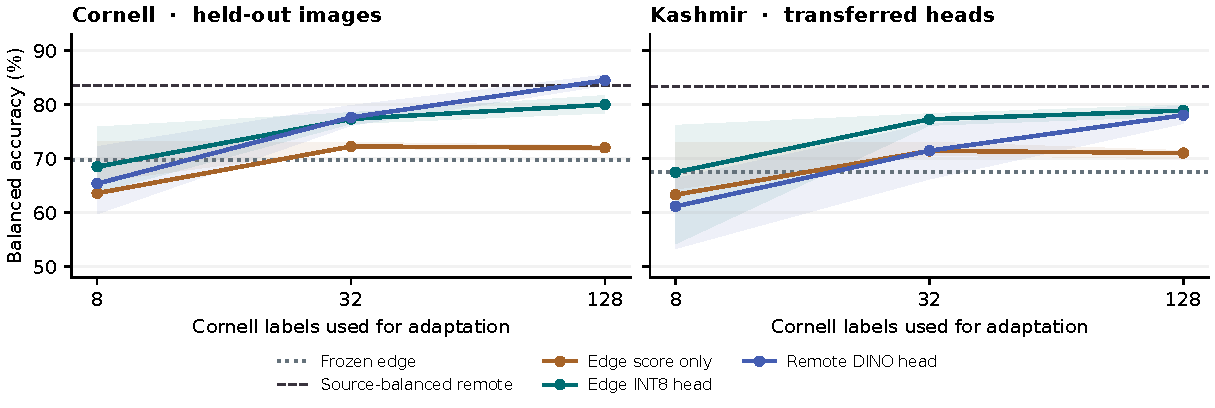
\includegraphics[width=.96\linewidth]{figures/adaptation.pdf}\end{center}
\note{Figure B1. Lines give means over the 20 draws. Shading gives the interquartile range. The same fitted heads are applied unchanged to the processed Kashmir pool. Dashed lines correspond to the source-balanced remote model.}

The INT8 head improves the score ordering. With 128 labels the mean AUROC increases by 14.80 points over the unchanged edge. The one-dimensional edge control retains its prior ordering at 32 and 128 labels. The independent host C99 implementation decoded all 60 packed INT8 heads and matched the Python class decisions on all 81,180 head--image pairs.

\newpage
\sect{Appendix C \quad When does an update use less communication?}
With labels available at the camera, 32 labelled activations and one returned head cost 42,670 bytes. At 128 labels the cost is 166,798 bytes. If a remote reviewer must inspect each calibration photograph, we charge its measured JPEG and identifier as well. The corresponding mean costs are 257,402 and 1,026,890 bytes. The fully remote target-fitted DINO pipeline reuses the same calibration images for review and training and processes every holdout picture. Its mean exchange totals 9,356,348 and 10,001,804 bytes, respectively, including application-level requests and replies. It achieves a higher mean BA at 128 labels. These costs are specific to 1,353 subsequent images.

\subt{A lower bound for the image-based alternative}
To avoid choosing a weak routing baseline, give a router the true class and let it choose the cheapest correcting option on every original edge error. The enlarged menu includes 112- and 224-pixel MobileNet, plus both DINO source heads at 224 pixels. Agreements and regressions can be skipped. Sort correcting payload sizes separately for healthy and diseased edge errors and form prefix costs $C_0(i)$ and $C_1(j)$. With $n_0,n_1$ examples per class, the minimum cost of a BA gain $g$ is
\[
 \min_{i,j}\; C_0(i)+C_1(j) \quad\text{subject to}\quad
               i/(2n_0)+j/(2n_1)\geq g.
\]
For given correction counts the cheapest prefixes attain the minimum, since replacing an expensive correctable image with a cheaper one of its class preserves BA. Enumerating the healthy prefix and the shortest feasible diseased prefix solves the finite problem. Exhaustive assignment on 72 small pools verified the implementation. The comparator even omits network headers and replies, favouring image routing.

\begin{center}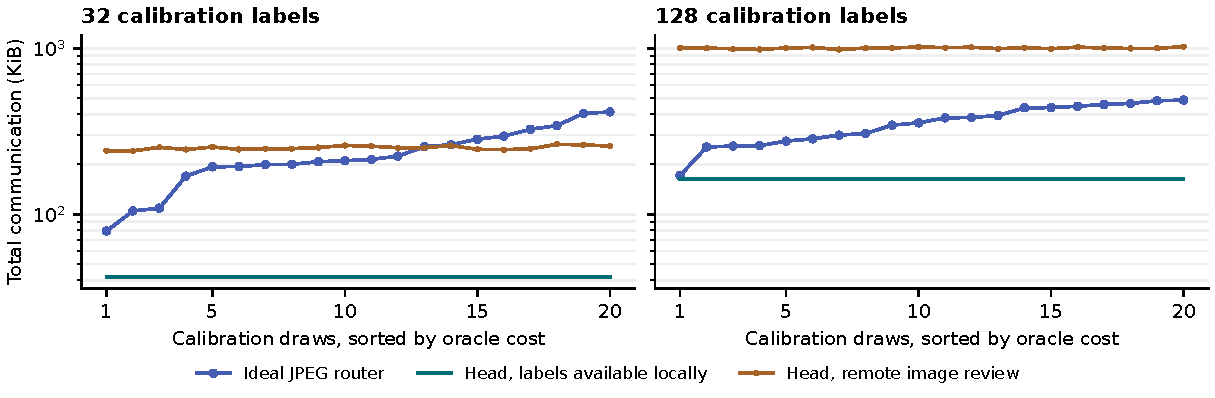
\includegraphics[width=.90\linewidth]{figures/oracle.pdf}\end{center}
\note{Figure C1. Bytes over the entire holdout to match each fitted INT8 head's achieved BA. An oracle can use labels to choose uploads. The two update curves differ only in where calibration images are reviewed.}

At 32 labels the median oracle cost was 217,018 bytes, compared with 42,670 for local review. At 128 it was 376,441 bytes, compared with 166,798. When all labels were available at the camera, the update beat the bound in all 20 draws at both budgets. Sending every calibration image to the annotator changed those counts to 8 of 20 at 32 labels and zero at 128. With 32 of 128 images sent, only 9 of 20 updates remained cheaper, declining to zero with 64 sent. The comparator covers the stated frozen menu and baseline edge. Models with different features, on-camera reweighting, or new encodings would require their own bound.

\subt{Batch service under recorded cellular capacity}
Three paired Mahimahi uplink/downlink traces \cite{mahi} provide 1,500 bytes per opportunity, with five initial phases. For 1,353 pending images, the update finished all 1,200 paired transfers sooner. For one image it won 600, tied 80 and lost 520. On AT\&T driving LTE with remote labels, median service for update versus full review was 8.294 versus 6.879 s (one pending image) or 8.294 versus 87.656 s (1,353). These are capacity-only estimates. Section 6 evaluates RTT, retransmission, outages, processing and deadlines separately.

\newpage
\sect{Appendix D \quad Which operating conditions change the answer?}
\subt{A deployment that prioritizes sensitivity}
The 128-label INT8 head increased healthy specificity from 42.97\% to 73.86\% on Cornell. Disease sensitivity declined from 96.52\% to 86.17\%. An operator for whom a missed lesion is much worse than an extra inspection would value these changes differently. We therefore divide each 128-label draw into 64 fitting and 64 threshold-calibration examples. For each fitted score we choose the largest threshold that accepts at least 95\% of calibration positives, using the inclusive order statistic. Between 41 and 51 positives contributed to each selected threshold.

\begin{center}\small
\begin{tabular}{@{}lrrrr@{}}\toprule
Held-out operation & Sens. (\%) & Spec. (\%) & BA (\%) & Draws at 95\% sens.\\\midrule
Frozen published cutoff &96.52&42.97&69.74&20/20$^{*}$\\
Original margin, calibrated cutoff &94.09&48.62&71.35&9/20\\
INT8 head, default cutoff &86.09&69.95&78.02&0/20$^{\dagger}$\\
INT8 head, calibrated cutoff &94.19&53.28&73.73&11/20\\
DINO target head, calibrated cutoff &92.07&64.97&78.52&2/20\\\bottomrule
\end{tabular}\end{center}
\note{$^{*}$The frozen classifier is repeated unchanged on the common holdout. $^{\dagger}$The default-cutoff entry is taken from the same 64-label fitting experiment as the calibrated entry.}

Adjusting only the original score threshold and fitting a scalar logistic function before thresholding gave identical decisions in all 20 runs. At the calibrated operating point, the adapted edge provided higher mean specificity than the margin-only baseline at similar average sensitivity. Individual fitted-head sensitivities ranged from 86.17\% to 98.57\%. A target sensitivity on the calibration panel did not certify it on the held-out images.

\subt{Transfer without local refitting}
The third collection comprises apple images acquired in Jammu and Kashmir \cite{yatoo}. A pinned public mirror has 5,612 processed rows with three classes. We took the 128 lowest salted filename hashes in each class. The 384 selected files had unique SHA-256 values and no perceptual match within the pool or against 7,191 checked source files, including Cornell. The originating collection uses augmentation, and parent photograph identities are unavailable in the mirror. Counts describe a finite processed-image pool. Sampling equal counts per source class gives twice as many diseased as healthy images in the binary task.

Transferred 128-label INT8 heads achieved 78.91\% mean BA versus 67.58\% for the frozen edge. Specificity rose from 36.72\% to 78.48\%, while sensitivity fell from 98.44\% to 79.34\%. Ordinary accuracy changed from 77.86\% to 79.05\%. A DINO head fitted to the same Cornell labels achieved 78.05\% BA on transfer. The source-balanced DINO model reached 83.40\% with no Cornell labels. These estimates apply to the V2 pipeline with supervision already available. The source-balanced remote model supplies the common expert for the experiments in Sections 3--5.

\subt{Scope of the device and network measurements}
Archived hardware validates the starting device model for only one fixed cohort. The preceding experiment fitted and evaluated heads on features of the frozen FP32 graph. Section 6 quantifies sensitivity to its numerical approximation. Their compute and energy on the deployed INT8 backbone remain unmeasured. Image-source labels are proxies for visible abnormality, with unknown plant-level groupings. Measured payloads and historical network traces support communication comparisons. Neither establishes end-to-end field latency, disease prevalence, yield improvement or effects of acting on an alert. For this camera and these collections, the operational choice turns on the reviewer location, cost of a miss, and number of future images over which one can amortize an update.

\newpage
\sect{Appendix E \quad Retrospective batch scheduling with local supervision}
An updated edge classifier can change both its answers and the order in which it asks for help. We gave every strategy the same ceiling in application bytes. A review transmits a real 224-pixel JPEG and 20 bytes of request and reply fields to the same frozen PlantDoc-balanced DINO service. Unqueried images keep their edge decisions. The original camera queues frames closest to its released 0.30 cutoff. The updated camera queues frames with the smallest absolute distance from its new logit cutoff of zero. The sender knows JPEG lengths after encoding and can buffer the batch. A frame is skipped if it does not fit in the remaining allowance. The scheduler sees no evaluation label or remote prediction before making that choice.

For this historical batch comparison we fixed a ceiling of 25\% of the bytes for full review, with 10\% and 50\% for sensitivity. The 20 Cornell-trained 128-label heads in Appendix~B are reused without refitting. We charge the complete calibration and deployment cost to each cohort, including both transfers. If an update cannot fit, the combined system uses the original edge router. The table assumes the 128 reference labels are available at the camera during Cornell calibration.

\begin{center}\small
\begin{tabular}{@{}lrrr@{}}\toprule
Mean BA (\%), 25\% ceiling unless marked & Cornell & Kashmir & Latvia\\\midrule
Frozen server on every image (100\% ceiling) &83.56&83.40&60.64\\
Original edge &69.74&67.58&46.90\\
Original edge + selective review &72.62&76.37&51.54\\
Updated edge alone &80.01&78.91&52.11\\
Updated edge + random review &80.85&79.75&54.55\\
Updated edge + selective review &\textbf{87.06}&\textbf{84.28}&\textbf{54.74}\\\bottomrule
\end{tabular}\end{center}
\note{Latvia uses the presence of visible scab as its endpoint. The random control uses 20 fixed image orderings for each of the 20 head draws and pays the same setup cost. Selective review used means of 283, 75 and 272 uploads (rounded).}

\begin{center}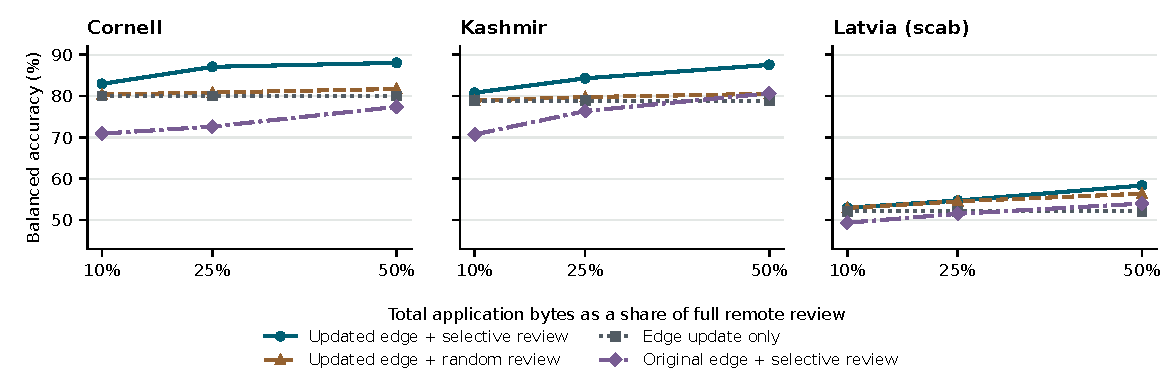
\includegraphics[width=.96\linewidth]{figures/collaboration.pdf}\end{center}
\note{Figure E1. Each cohort uses its own byte ceiling. Each mean reuses a single evaluation pool across draws. The line for the update alone falls back to the original camera if the update cannot fit.}

On Cornell and Kashmir, every calibration draw beat both single interventions at 25\%. The selective policy corrected 100.45 and spoiled 33.35 Cornell decisions per draw, compared with the updated edge alone. On Kashmir these values were 24.65 and 8.20. On Latvia the selective and random policies were within 0.19 points, and only 10 of 20 draws beat mean random review. The service corrected 51.45 decisions and spoiled 91.55 on average there. With 207 negatives and 983 positives there, ordinary accuracy fell from 73.70\% for the original camera to 48.67\% for the joint policy. Mean scab misses rose from 118 to 536.35.

If the Cornell calibration photographs must be transmitted for annotation, joint BA at 25\% becomes 84.76\%, 76.37\% and 53.70\%, respectively. On Kashmir the mean calibration exchange alone exceeded the entire 945,647-byte allowance in every draw. Paying for the labels eliminates the update at this ceiling.

\newpage
\sect{Appendix F \quad Can full review reduce false alarms and misses together?}
Changing one cutoff on a fixed ordering adds or removes alerts in a single direction. To examine two independent changes, we allowed the source-balanced remote model to rescue an edge-negative image and to retract an edge-positive alert. A 475-rule grid was fixed before examining results for this policy. We used the 450 Cornell calibration images to require at least a halving of the 15 original misses and fewer than the 83 original false positives. Four rules qualified. Prespecified tie-breaking first minimized false positives. The selected rule yielded 60 false positives and five misses on calibration. Earlier methods had already been evaluated on the Cornell and Kashmir test collections.

The selected rule queried every photograph. For an original negative it issues an alert if the service's estimated disease probability is at least 0.50. For an original positive it clears the alert only below 0.30. Fitting required 3,031,861 calibration bytes, followed by a 22-byte configuration. All deployments below replay the very same configuration.

\begin{center}\small
\begin{tabular}{@{}lrrr@{}}\toprule
Source and reference counts & False positives & False negatives & Inference bytes\\\midrule
Cornell (377 negative, 976 positive) &$215\to137$&$34\to19$&9,141,584\\
Kashmir (128 negative, 256 positive) &$81\to25$&$4\to25$&3,782,589\\
Latvia (207 negative, 983 positive) &$195\to83$&$118\to334$&10,788,080\\\bottomrule
\end{tabular}\end{center}

The Cornell rule corrected 108 false alarms and 25 missed cases, while introducing 30 false alarms and 10 misses. Much of its net rescue came from scab, where misses fell from 21 to four. Among 67 images with multiple diseases, misses increased from one to four. In Kashmir, 22 of the 24 introduced misses occurred on Alternaria. Only three originally missed Kashmir cases were rescued. These counts come from the same image decisions and distinguish the type of mistake that moved the average.

\subt{Competing choices of representation and operating point}
On Cornell, a single 448-pixel JPEG with three DINO views, fitted on 300 Cornell examples and thresholded on the remaining 150 calibration examples, yielded 83 false positives and 38 misses at a cost of 26,528,371 inference JPEG bytes. On Kashmir it yielded four and 75 respectively. On Latvia it yielded 37 and 401. A preselected two-score fusion yielded 120/39, 22/33 and 64/404, respectively (false positives/misses). Using more pixels or adding two scores can suppress false alarms while losing the intended sensitivity.

Two of 20 earlier high-sensitivity INT8 heads (draws 2 and 4) reduced both counts on both Cornell and Kashmir. They were identified after examining those results. Both were then fixed for Latvia, where their error counts were 192/126 and 181/164, respectively, against the original 195/118. Conditional selection would have overstated their portability.

A stronger single-expert control received the identical 450 labels and considered every distinct observed remote-score cutoff and its endpoints. Under the common calibration constraint of at most seven misses it selected 0.33966 (63 false positives and five misses). In full review it gave 173/18 on Cornell, 25/34 on Kashmir and 62/359 on Latvia. Against this control, the directional combination eliminated nine further misses at unchanged false positives on Kashmir. In Latvia it exchanged 21 additional false positives for 25 fewer misses. The fixed 0.50 remote model also retained higher Cornell BA than the directional combination (83.56\% versus 80.86\%). Threshold comparisons and both single-score controls are included in the artifact. The two-score rule's value depends on the cost assigned to each error.


\newpage
\sect{Appendix G \quad External scab screening and local recalibration}
AppleScabLDs contains all 1,190 leaf photographs in the specified Latvian archive \cite{kodors}, with 207 publisher-negative and 983 visible-scab references. An image without visible scab can show other damage. Photographs include repeated leaf views. An independent ZIP traversal verified all paths, SHA-256 values, labels and perceptual hashes. No exact or perceptual match within Hamming distance five was found against 7,575 archived source images. In the Latvian archive, one member per same-label component at distance four yields 1,148 representatives. The fixed Cornell rule changes false positives from 191 to 81 and misses from 116 to 324 on this subset. Neither perceptual grouping nor spatially distinct collections establishes leaf-level statistical independence.

All images retained original capture dates over 14 days. We reserved the earliest five full days for calibration and all nine later days for evaluation, before looking at the new predictions. No exact or screened near-duplicate component crossed these two partitions. The five days supplied 611 images and labels, including 476 with scab. The later days contained 72 negatives and 507 positives. The date split therefore required substantially more calibration images than a one-third split of individual files.

The identical 475-rule procedure found no candidate that halved calibration misses while lowering false positives. Its prespecified fallback chose among the 38 rules that strictly lowered both. It changed early error counts from 128/69 to 126/56. On the 579 later images the baseline had 67 false positives and 49 misses. The Cornell rule yielded 30 and 159. The rule calibrated on the five local dates yielded 67 and 33. It rescued 18 missed scab images and incorrectly withdrew two true alerts. Sensitivity rose from 90.34\% to 93.49\%, while specificity remained 6.94\%. The early labels and rule installation cost 5,497,944 bytes, followed by 1,554,379 bytes for 175 later queries. This is a within-season analysis with a small later negative cohort.

\begin{center}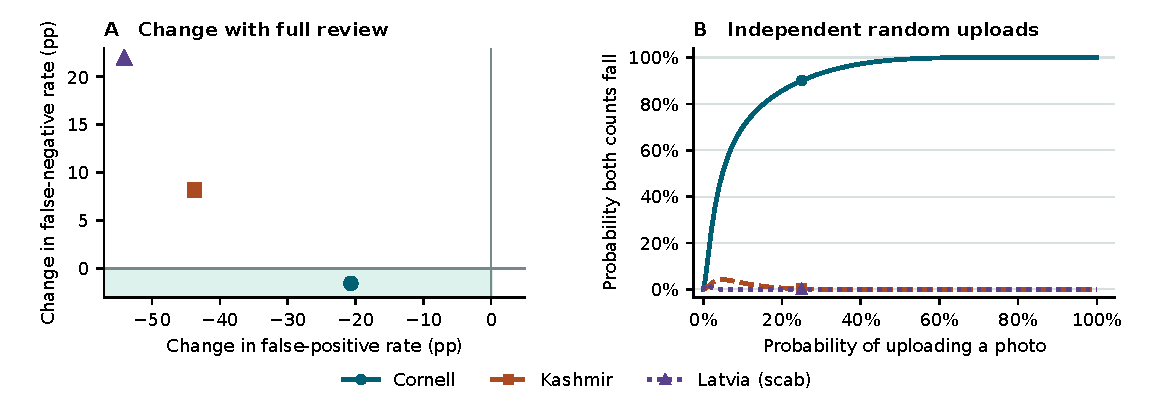
\includegraphics[width=.96\linewidth]{figures/joint_errors.pdf}\end{center}
\note{Figure G1. Left, the shaded quadrant denotes strictly fewer errors in both classes. Right, for a fixed set of scored images, the only randomness is an independent decision to upload each eligible image with probability $q$. At $q=1$ all eligible images get the full-review treatment.}

If full review fixes $a$ and spoils $b$ decisions of one true class, independently sampling eligible uploads with probability $q$ gives a strict improvement probability $P[\mathrm{Bin}(a,q)>\mathrm{Bin}(b,q)]$ for that class, using two independent binomials. The two class-specific events involve disjoint uploads, so their probabilities multiply. At $q=0.25$ the probability of a strict joint reduction is 90.05\% on the fixed Cornell batch and 0.23\% on the fixed Kashmir batch. This retrospective calculation quantifies routing randomness. It assumes no probability law for new leaves.

\end{document}
